\documentclass[mathserif]{beamer} % New pstricks (otherwise add [xcolor=pst])
\usepackage{etex}
\usepackage{amsmath,amssymb,latexsym,amsthm}
\usepackage{pstricks}
\usepackage{pst-plot,animate,hyperref}
\usepackage{graphicx,subfigure}
\graphicspath{{../../figs/}{../../Fig/}}
\usepackage{float,rotating,mdframed}
\usepackage{comment,color}
%\usepackage{multimedia}
\usepackage{movie15}

\definecolor{palegray}{rgb}{0.9,0.9,0.9} 
\def\pitem{\pause\item}
\newcommand{\id}{\,\mathrm{d}}
\newcommand{\di}{\partial}
\newcommand{\vc}{\mathbf}
\newcommand{\charf}{\raisebox{\depth}{\(\chi\)}}
\newcommand{\F}{F_{t_0}^t}
\newcommand{\C}{C_{t_0}^t}
\newcommand{\D}{D_{t_0}^t}
\newcommand{\bnabla}{\pmb\nabla}
\newcommand{\bxi}{\pmb\xi}
%\newcommand{\pitem}{\pause\item}
%-------------------------------------------------------
\usetheme{default}
\mode<presentation>
{
  \usetheme{default}
%  \setbeamercovered{transparent} %--Show covered items in grey
  \setbeamertemplate{navigation symbols}{} %--Do not show navigation symbols
}
%------------------------------------------------
\title[]
{Adjoint equation for computing equilibrium solutions of Navier--Stokes equation:\\ 
Towards high Reynolds numbers}
\author[Mohammad Farazmand]{{\bf Mohammad Farazmand, Predrag Cvitanovi\'c}}
%
\institute[Georgia Tech]
{Center for Nonlinear Science\\ School of Physics, Georgia Institute of Technology\\
  \includegraphics[width=0.3\textwidth]{gatech_logo}\\
  \textcolor{blue}{SIAM Conference on Applications of Dynamical Systems}
}
\date{\tiny May 18, 2015}
%
\begin{document}
\begin{frame}
  \titlepage
\end{frame}
%
\begin{frame}
\frametitle{Motivation}
Steady and recurrent solutions form the backbone of turbulence\\
\ \\
\begin{columns}
\column{.5\textwidth}
\centering
\includegraphics[width=\textwidth]{Walleffe_PhyFluids2003}\\
{\tiny \textcolor{blue}{F. Waleffe, Phys. Fluids (2003)}}
\column{.5\textwidth}
\centering
\includegraphics[width=\textwidth]{GC_JFM08}\\
{\tiny \textcolor{blue}{Gibson, Halcrow \& Cvitanovi\'c, JFM (2008)}}
\end{columns}
%
\begin{columns}
\column{.6\textwidth}
\begin{itemize}
\item {\small Geometry of the state space}\\
\item {\small Quantitative predictions:\\ Periodic orbit theory}\\
{\tiny \textcolor{blue}{Cvitanovi\'c et al., Chaosbook.org}}\\
{\tiny \textcolor{blue}{Chandler \& Kerswell JFM (2013)}}
\end{itemize}
\column{.4\textwidth}
\centering
\includegraphics[width=\textwidth]{GHC_JFM08_ss}\\
{\tiny \textcolor{blue}{Gibson, Halcrow \& Cvitanovi\'c, JFM (2008)}}
\end{columns}
\vspace{.5cm}
Open access code: \texttt{channelflow.org} \& \texttt{openpipeflow.org}
\end{frame}
%
\begin{frame}
\frametitle{History}
\begin{itemize}
	\item {\small First steady solutions of plane Couette flow (PCF)}\\
	{\tiny \textcolor{blue}{M. Nagata JFM (1990)}}
	\item {\small First traveling wave solutions of PCF}\\
	{\tiny \textcolor{blue}{M. Nagata PRE (1997)}}
	\item {\small First (relative) periodic solutions of PCF}\\
	{\tiny \textcolor{blue}{G. Kawahara, \& S. Kida JFM (2001), D. Viswanath JFM (2007)}}
\end{itemize}
And many many more:\\
{\tiny \textcolor{blue}{Willis \& Kerswell, PRL (2008)}}\\
{\tiny \textcolor{blue}{Viswanath, Phil. Trans. R. Soc. A (2009)}}\\
{\tiny \textcolor{blue}{Willis, Cvitanovi\'c \& Avila, JFM (2013)}}\\
{\tiny \textcolor{blue}{Gibson \& Brand, JFM (2014)}}
\end{frame}
%
\begin{frame}
\frametitle{Continuous-time Newton descent}
\tiny{\textcolor{blue}{``This geometry is based on an idea which is known, but not usually explicated. Namely, Newton's method for solving $f(z)=0$ is an Euler approximation to the ordinary differential equation...", Steve Smale (1981)}}
\normalsize
$$\partial_t\vc u =\vc F(\vc u),\quad \vc u=\vc u(\vc x,t)$$
Equilibrium solutions: $$\vc F(\vc u_0)=\vc 0$$
\pause
Consider a second PDE 
$$\partial_\tau \vc u =\vc G(\vc u)$$
$$\pmb{\mathcal L}(\vc u;\vc G(\vc u))=-\vc F(\vc u)$$
where $\pmb{\mathcal L}$ is the G\^ateaux derivative
$$\pmb{\mathcal L}(\vc u;\vc v)=\lim_{\epsilon\to 0}\frac{\vc F(\vc u+\epsilon\vc v)-\vc 
F(\vc u)}{\epsilon}$$
%such that 
%$$\|\vc F(\vc u(\tau))\|\to 0\quad \mbox{as} \quad \tau\to \infty$$
%\pause
%Note that
%$$\partial_\tau\|\vc F(\vc u(\tau))\|^2=2\langle \pmb{\mathcal L}(\vc u;\vc G(\vc 
%u)),\vc 
%F(\vc u)\rangle$$
\pause
Then 
$$\|\vc F(\vc u(\tau))\|=\|\vc F(\vc u(0))\|\exp(-\tau)$$
\end{frame}
%
\begin{frame}
\frametitle{Discrete Newton descent}
$$\partial_\tau \vc u =\vc G(\vc u)$$
$$\pmb{\mathcal L}(\vc u;\vc G(\vc u))=-\vc F(\vc u)$$
\hrule\ \\
\pause
$$\vc A(\tilde{\vc u})\tilde{\vc G}=-\tilde{\vc F}(\tilde{\vc u})$$ 
\begin{itemize}
\item
The descent direction $\tilde{\vc G}$ is approximated by Newton-GMRES iterations 
[\alert{costly in high dimensions}]
\pause\item 
State $\tilde{\vc u}$ is updated by discrete Newton iterations:
$$\tilde{\vc u}_{i+1}=\tilde{\vc u}_i -\delta\tau\;\tilde{\vc G}_i$$
\pause\item 
Super-exponential convergence \alert{if a good initial guess is provided}
\end{itemize}
\end{frame}
%
\begin{frame}
\frametitle{Adjoint descent}
\begin{align*}
\partial_\tau\|\vc F(\vc u(\tau))\|^2& =2\langle \pmb{\mathcal L}(\vc u;\vc G(\vc u)),\vc 
F(\vc u)\rangle\\
 & =2\langle \vc G(\vc u),\pmb{\mathcal L}^\dagger(\vc u;\vc F(\vc u))\rangle
\end{align*}
\pause
Let 
$$\vc G(\vc u)=-\pmb{\mathcal L}^\dagger(\vc u;\vc F(\vc u))$$
\begin{itemize}
\pause\item The adjoint operator can be computed explicitly.
\pause\item Integration of $\partial_\tau \vc u=\vc G(\vc u)$ with higher accuracy is 
feasible.
\pause\item Convergence is `guaranteed' but the rate of convergence may be slow.
\end{itemize}
{\tiny\textcolor{blue}{J. Yang \& T.I. Lakoba, Stud. Appl. Math (2007)}, Nonlinear Schr\"odinger and Ginzburg--Landau equations}
\end{frame}
%
\begin{frame}
\frametitle{Adjoint equation for Navier--Stokes}
Navier--Stokes equation:
$$\partial_t\vc u=-\vc u\cdot\bnabla\vc u\textcolor{red}{-\bnabla p} +\nu \Delta \vc u 
+\vc f(\vc x),
\quad \bnabla\cdot\vc u=0$$
$$\vc x=\mathbb T^3=[0,2\pi]\times[0,2\pi]\times[0,2\pi]$$
\pause
Seek the adjoint equation over the function space\\
\begin{center}
$\mathcal H=\{\vc u(\cdot,t)\in L^2(\mathbb T^3):
\bnabla\cdot \vc u(\cdot,t)=0 \}$
\end{center}
\pause
Treating the div-free condition as a Lagrange multiplier:
$$\partial_\tau\vc u = -\left\{\left[\bnabla\vc F+(\bnabla\vc F)^\top\right]\vc 
u-\bnabla p'+\nu\Delta \vc F\right\}$$
$$\vc F=\vc F(\vc u) := -\vc u\cdot\bnabla\vc u -\bnabla p +\nu\Delta\vc u+\vc 
f(\vc x)$$
$$\bnabla\cdot\vc F=0,\quad \bnabla\cdot\vc u=0$$
{\tiny\textcolor{blue}{M. Farazmand \& P. Cvitanovi\'c, preprint (2015)}}
\end{frame}
%
\begin{frame}
\frametitle{Kolmogorov flow}
{\tiny \textcolor{blue}{Chandler \& Kerswell, JFM (2013), Lucas \& Kerswell, JFM (2014)}}
$$\partial_t\vc u=-\vc u\cdot\bnabla\vc u-\bnabla p +\nu \Delta \vc u +\sin(ny)\vc e_1$$
$$\bnabla\cdot\vc u=0$$
$$\vc u(x,y,t)=(u_1(x,y,t),u_2(x,y,t))\in\mathbb R^2$$
$$(x,y)\in\mathbb T^2=[0,2\pi]\times[0,2\pi]$$
\pause
Laminar solution:
$$u_1=\frac{Re}{n^2}\sin(ny),\quad u_2=0,\quad Re=1/\nu$$
\pause
Energy Dissipation and Input:
$$D(t)=\frac{1}{Re}\langle|\bnabla\vc u|^2\rangle,\quad I(t)=\langle 
u_1(x,y,t)\sin(ny)\rangle$$
For equilibria: $D(t)=I(t)=\mbox{Constant}$
\end{frame}
%
\begin{frame}
\frametitle{Error analysis}
$Re=40$,\hspace{.5cm} Initial guess $\vc u(x,y)=(2\cos(2y),2\cos(2x))$
\begin{figure}
\centering
\includegraphics[width=.75\textwidth]{Kol_R40_n64_err_E1}
\end{figure}
\textcolor{blue}{Pure Newton-GMRES iterations}\\
\textcolor{red}{Adjoint Eq. integrated for $\tau=5$ $\quad\simeq 13$ seconds}\\
\textcolor{black}{6 Newton-GMRES iterations $\quad\quad\;\;\,\simeq 58$ seconds}
\end{frame}
%
\begin{frame}
	\frametitle{Example}
	$Re=40$, Resolution $128\times 128$\\ \vspace{.5cm}
	\begin{columns}
		\column{.33\textwidth}
		\centering
		\includegraphics[width=\textwidth]{Kol_R40_n128_vort_E2_t0}
		\column{.33\textwidth}
		\centering
		\includegraphics[width=\textwidth]{Kol_R40_n128_vort_E2_adj_t5e3}
		\column{.33\textwidth}
		\centering
		\includegraphics[width=\textwidth]{Kol_R40_n128_vort_E2}
	\end{columns}
	\ \\
	{\tiny 
		\begin{columns}
			\column{.33\textwidth}
			\centering
			Initial condition\\ $\vc u(x,y)=(2\cos(2y),2\cos(2x))$
			\column{.33\textwidth}
			\centering
			Solution of the adjoint at $\tau = 5$\\ ($13$ seconds)
			\column{.33\textwidth}
			\centering
			After $6$ Newton-GMRES iterations converged with residue $<10^{-10}$\\ ($58$ seconds)
		\end{columns}
	}
\end{frame}
%
\begin{frame}
\begin{figure}
\centering
\includegraphics[width=.9\textwidth]{ID_R40_mod}
\end{figure}
\end{frame}
%
\begin{frame}
\frametitle{Intermittency}
\begin{columns}
\column{.45\textwidth}
\centering
%\movie[loop,width=\textwidth,hight=.9\textwidth]{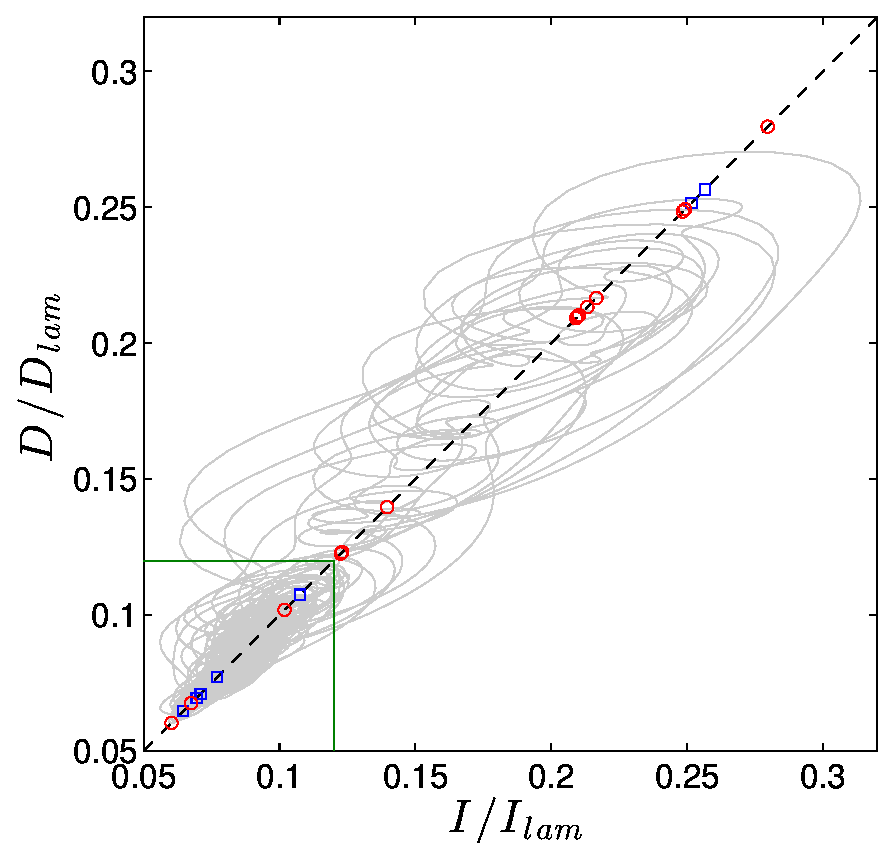
\includegraphics[width=.9\textwidth]{ID_R40}}{ID_R40_comp.mov}
\includemovie[rate=4,playerid=AAPL_QuickTime,text={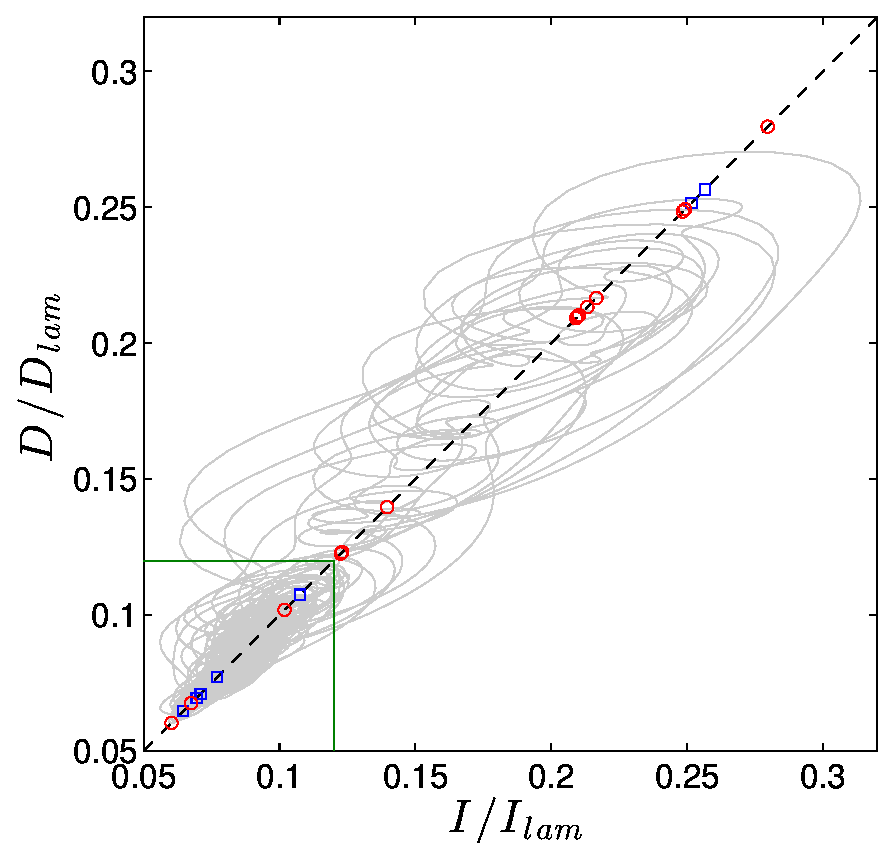
\includegraphics[width=.9\textwidth]{ID_R40}}]{\textwidth}{.9\textwidth}{ID_R40_comp.mov}
\column{.55\textwidth}
\includegraphics[width=\textwidth]{intermittency_R40}
\end{columns}
%
%\pause
%\begin{columns}
%\column{.5\textwidth}
%\centering
%\includegraphics[width=.65\textwidth]{Kol_R40_erg_vort_t242}\\
%{\tiny Ergodic trajectory at $t=242$}
%\column{.5\textwidth}
%\centering
%\includegraphics[width=.65\textwidth]{Kol_R40_n128_vort_E2}\\
%{\tiny Equilibrium solution with $D/D_{lam}=2.13\times 10^{-1}$}
%\end{columns}
\end{frame}
%
\begin{frame}
\textcolor{blue}{Conclusions}
\begin{itemize}
\item Adjoint equation for computing equilibria of NS
\item Speed up in convergence
\item Converges with bad initial guesses $\Rightarrow$\\ More equilibrium solutions
\item Straightforward implementation with pseudo-spectral methods
\end{itemize}
\pause\textcolor{blue}{Future work:}
\begin{itemize}
\item Discretization scheme for NS with boundary conditions
\item Higher Reynolds numbers $\Rightarrow$ HPC\\
\centering
\includegraphics[width=.35\textwidth]{Kol_R100_n256_vort_E4-2sin}\hspace{.5cm}
\centering
\includegraphics[width=.35\textwidth]{Kol_R100_n256_vort_E2}
\begin{center}
	$Re=100$
\end{center}
\item Feasibility for unstable periodic orbits {\tiny\textcolor{blue}{J. Yang, 
Stud. Appl. Math. (2015)}}
\end{itemize}
\end{frame}

\end{document}